\documentclass[conference]{IEEEtran}
\usepackage{amsfonts}
%\usepackage{amsthm}
\usepackage{graphicx}
%\usepackage{fancyhdr}
%\usepackage{floatflt}
\usepackage{cite}
\usepackage{balance}

\flushbottom

\setlength{\parindent}{1em}
\setlength{\parskip}{.15em}
\setlength{\oddsidemargin}{0in}
\setlength{\textwidth}{6.5in} % sets 1in left and right margins
\setlength{\topmargin}{0.20in} % change to 0.2in for regular latex
%\setlength{\headheight}{0in}
%\setlength{\footheight}{0.5in}
\setlength{\footskip}{0.5in}
\setlength{\textheight}{9.0in} %sets 1in top and bottom margins
\renewcommand{\baselinestretch}{1} %set to 1.5 for double spacing.

\newcommand{\br}{{\mathbf r}}
\newcommand{\bA}{{\mathbf A}}
\newcommand{\ba}{{\bf a}}
\newcommand{\bb}{{\bf b}}
\newcommand{\bc}{{\bf c}}
\newcommand{\bC}{{\bf C}}
\newcommand{\bg}{{\bf g}}
\newcommand{\bG}{{\bf G}}
\newcommand{\bd}{{\bf d}}
\newcommand{\be}{{\bf e}}
\newcommand{\bq}{{\bf q}}
\newcommand{\bs}{{\bf s}}
\newcommand{\bm}{{\bf m}}
\newcommand{\bn}{{\bf n}}
\newcommand{\bu}{{\bf u}}
\newcommand{\bv}{{\bf v}}
\newcommand{\bw}{{\bf w}}
\newcommand{\bx}{{\bf x}}
\newcommand{\by}{{\bf y}}
\newcommand{\bz}{{\bf z}}
\newcommand{\bbf}{{\bf f}}
\newcommand{\bE}{{\bf E}}
\newcommand{\bF}{{\bf F}}
\newcommand{\bL}{{\bf L}}
\newcommand{\bM}{{\bf M}}
\newcommand{\bN}{{\bf N}}
\newcommand{\bS}{{\bf S}}
\newcommand{\bT}{{\bf T}}
\newcommand{\bD}{{\bf D}}
\newcommand{\bX}{{\bf X}}
\newcommand{\bP}{{\bf P}}
\newcommand{\bQ}{{\bf Q}}
\newcommand{\bI}{{\bf I}}
\newcommand{\bR}{{\bf R}}
\newcommand{\bU}{{\bf U}}
\newcommand{\bV}{{\bf V}}
\newcommand{\bW}{{\bf W}}
\newcommand{\bY}{{\bf Y}}
\newcommand{\bZ}{{\bf Z}}
\newcommand{\bJ}{{\bf J}}
\newcommand{\bB}{{\bf B}}
\newcommand{\bzero}{{\bf 0}}
\newcommand{\bgamma}{{\mbox {\boldmath $\gamma$}}}
\newcommand{\btheta}{{\mbox {\boldmath $\theta$}}}
\newcommand{\bLambda}{{\mbox {\boldmath $\Lambda$}}}
\newcommand{\bPsi}{{\mbox {\boldmath $\Psi$}}}
\newcommand{\bPhi}{{\mbox {\boldmath $\Phi$}}}
\newcommand{\bphi}{{\mbox {\boldmath $\phi$}}}
\newcommand{\bpsi}{{\mbox {\boldmath $\psi$}}}
\newcommand{\bcA}{{\mbox {\boldmath ${\cal A}$}}}
\newcommand{\bcB}{{\mbox {\boldmath ${\cal B}$}}}
\newcommand{\bcC}{{\mbox {\boldmath ${\cal C}$}}}
\newcommand{\bcD}{{\mbox {\boldmath ${\cal D}$}}}
\newcommand{\bcF}{{\mbox {\boldmath ${\cal F}$}}}
\newcommand{\bcN}{{\mbox {\boldmath ${\cal N}$}}}
\newcommand{\bcR}{{\mbox {\boldmath ${\cal R}$}}}
\newcommand{\bcS}{{\mbox {\boldmath ${\cal S}$}}}
\newcommand{\bcH}{{\mbox {\boldmath ${\cal H}$}}}
\newcommand{\bcI}{{\mbox {\boldmath ${\cal I}$}}}


\begin{document}

\title{Blind Multiuser Receiver Design in ISI Channels}
%\author{Shu Wang and James Caffery, Jr.}
\author{\authorblockN{Shu Wang}
\authorblockA{LG Electronics Mobile Research\\
San Diego, CA 92131-1807\\
\em Email: swang@lge.com} \and
\authorblockN{James Caffery, Jr.}
\authorblockA{University of Cincinnati\\
Cincinnati, OH 45221-0030\\
\em Email: jcaffery@ececs.uc.edu}}

\maketitle
\begin{abstract}\small
In this paper, we present an alternative multiuser signal model
and discuss its applications for blind multiuser receiver design.
We compare the model with the conventional  and
signal subspace-based signal models as well as their applications
in receiver design. The geometric interpretation, bit-error rate,
signal processing bounds, etc., of these signal models and blind
receivers are compared and discussed.  From the analyses,
the trade-offs between the complexity and performance of blind
multiuser receiver design are presented. Computer simulations
are finally provided to demonstrate the performance and theoretic
analysis.
\end{abstract}

\section{Introduction}
The multiuser signal model not only enables understanding of signal
structures but also plays a key role in multiuser receiver design.
Multiuser detection (MUD) is a proven strategy for mitigating multiple
access interference (MAI) effects and limiting the near-far problem
by exploiting interference signal structure. MUD has received considerable attention over the past several years since MAI is the dominant
impairment for CDMA systems and even exists in the systems with
perfect power control~\cite{Verd98}.  It is believed to be one
of the critical techniques for enabling the high reliability and throughput of next-generation mobile communication systems~\cite{Andr05}. Most recent
research on MUD has been devoted to blind detection and subspace-based signature
waveform or channel estimation to reduce computational complexity and prior
knowledge requirements~\cite{Honi95,Torl97,Wang98,Zhang02,Wang03d,Wang05A,Wang05B}.
Blind multiuser receivers can achieve good performance given
knowledge of only the desired user's timing and signature waveform.
Such limited knowledge is much closer to practical applications than conventional methods since information about the interference (i.e., timing, signal structure, channel gains, etc.) is typically unknown beforehand. However, most
existing blind receivers are known to be too complicated for
high-data-rate applications.

In the development of advanced multiuser receivers, it is
known that a proper received signal model aids the understanding of
received signals as well as receiver design. There are two popular
multiuser signal models which have been extensively discussed for
multiuser receiver design. They are the conventional multiuser
signal model and the subspace-based multiuser signal model. In the
conventional signal model, each received signal is directly taken
as a linear combination of actual signal
signatures~\cite{Verd98,Honi95,Zhang02}.  Most related blind
multiuser receivers are developed either by explicitly estimating
the signal signature~\cite{Torl97} or by removing interfering
signal components using adaptive filtering techniques, e.g.,
blind receiver design with Wiener~\cite{Honi95} and Kalman
filter~\cite{Zhang02} techniques.  Though the conventional signal
model provides a natural view of received signals, the involved
signature waveforms and/or amplitude information are unknown and require considerable processing to obtain before detection.  To compensate for
the weakness of the conventional signal model, the subspace signal model was developed with subspace-based signal processing techniques~\cite{Wang98}. In the
subspace signal model, each received signal is taken as a linear
combination of signal subspace bases, which can be obtained by
subspace signal processing techniques on the autocorrelation
matrix of the received signals.  The subspace signal model can be considered a
result of parametric signal modeling and provides an in-depth
description of the received signals. Though the subspace-based
approach does not require explicit estimation of each user's
signature waveform and the adaptive speed is improved
with good performance, the signal subspace formation procedure
is not trivial.

While the conventional signal model provides a foundation for both
optimal and conventional multiuser receiver design and the subspace
signal model aids understanding of the underlying signal structure, neither
is simple enough for developing blind multiuser receivers for high-speed CDMA
systems~\cite{Andr05}. In order to address the near-far problem with
minimum prior knowledge and computational complexity, we propose a
new blind multiuser model by directly using current and past
received signal vectors with no explicit signal structure estimation.
With this blind signal model and widely employed signal estimation criteria including least squares (LS), minimum mean-squared error (MMSE), etc., several novel blind multiuser receivers are
developed. No statistical signal estimation or subspace
separation procedure is required. Only a minimum number of previously
received signals and the desired user's signature waveform
and timing are required. Hence, the computational complexity and
detection delay can be reduced.  We then compare the proposed blind
signal model and receivers with the conventional and subspace signal
models and the blind receivers based on them.  The trade-off between the performance and complexity in blind receiver development is discussed as well.  Computer simulations are provided to illustrate performance.

%%%%%%%%%%%%%%%%%%%%%%%%%%%%%%%%%%%%%%%%%%%%%%%%%%%%%%%%%%%%%%%%%
\section{Multiuser Signal Models}

Forward-link transmission in a single-cell DS/CDMA system
with $K$ active users is considered. The channel is a multipath
channel with $P$ resolvable paths and corrupted by additive white
Gaussian noise (AWGN).  The baseband representation of the received
signal due to user $k$ is given by
\begin{equation}
\begin{array}{l}\hspace{-0.2in}
r_k(t)=\sum\limits_{p=1}^{P}\alpha_{pk}A_k[n]
b_k[n]c_k(t-nT-\tau_p)+n_k(t)
\end{array}
\end{equation}
where $\alpha_{pk}$ is the gain of the $p$th path of user $k$'s
signal and $b_k{[n]}$ is the $n$th bit sent by user $k$. We assume
that the $\left\{b_k{[n]}\right\}$ are independent and identically
distributed random variables with $E\left\{b_k{[i]}\right\}=0$ and
$E\left\{|b_k{[i]}|^2\right\}=1$. The parameters $c_k(t)$ denote
the normalized spreading signal waveform of user $k$ during the
interval $[0,\ T]$ and $A_k[n]$ is the signal amplitude for user
$k$ at time $t=nT$.  Without loss of generality, the $P$ transmission delays from the base station to user $k$ are ordered such that $0\leq\tau_1\leq\tau_2\leq\ldots\leq\tau_P$.  The total baseband signal received for user $k$ is
\begin{equation}
\begin{array}{rcl}
\tilde{r}(t)&=&\sum\limits_{k=1}^{K}r_k(t) \enspace .
\end{array}
\end{equation}
The received signal $\tilde{r}(t)$ is passed through the
corresponding chip matched filter (CMF), $\phi(t)$, and RAKE
combiner. The combined output $r(t)$ is\footnote{Without loss of
the generality, we drop the time index $n$ in the following
discussion.}
\begin{equation}\hspace{-0.0in}
\begin{array}{rcl}
r(t)&=&A_k b_k c_k(t-nT-\tau_1)\otimes \phi(t-\tau_1) \\
&&\hspace{0.2in} + m_{\rm ISI}(t) + m_{\rm MAI}(t) + n(t)
\end{array}\label{r_t}
\end{equation}
where
\begin{equation} \hspace{-0.05in}
\begin{array}{rcl}
 m_{\rm ISI}(t)&=&\\
 &&\hspace{-0.83in}\sum\limits^{p,q=P}_{q\neq
p}\beta_{qk} \alpha_{pk}A_kb_kc_k(t-nT+\tau_{q1}-\tau_1)\otimes
\phi(t-\tau_1)
\end{array}
\end{equation}
is the intersymbol interference (ISI) to user $k$,
\begin{equation} \hspace{-0.05in}
\begin{array}{l}
m_{\rm MAI}(t)=\sum\limits_{i\neq
 k}^{K}A_ib_ic_i(t-nT-\tau_1)\otimes\phi(t-\tau_1)+\\
 \hspace{.0in}\sum\limits_{i\neq
 k}^{K}\sum\limits^{p,q=P}_{q\neq
p}\beta_{qk}
\alpha_{pi}A_ib_ic_i(t-nT+\tau_{q1}-\tau_p)\otimes\phi(t-\tau_1)
\end{array}
\end{equation}
\noindent is the MAI to user $k$, $\beta_{qk}$ is the weight of
the $q$th RAKE finger with
\begin{equation}
\begin{array}{rcl}
\sum\limits_{q=1}^{P}\beta_{qk}\alpha_{qk}&=&1
\end{array}
\end{equation}
and $\tau_{q1} = \tau_{q}-\tau_1$ is the propagation
delay difference between the first path and $p$th path and
$n(t)$ is AWGN with variance $\sigma^2$.  The symbol $\otimes$
denotes the convolutional product.  Because of $m_{\rm MAI}(t)$ in the received
signal, the performance of the conventional matched filter
receiver suffers from the  near-far problem~\cite{Verd98}.

%%%%%%%%%%%%%%%%%%%%%%%%%%%%%%%%%%%%%%%%%
\subsection{Conventional Signal Model}

After RAKE combining,  user $1$'s output can be sampled at rate
$f_s=1/T_s$ and expressed in vector notation by\footnote{Without loss of
the generality, we consider the first user as the desired user.}
\begin{eqnarray}
\br & = & \left[ r(nT+T_s+\tau_1),\ldots,r(nT+LT_s+\tau_1) \right]^{\rm
T} \nonumber \\
 &=&\sum\limits_{k=1}^{K} A_k b_k \bs_k + \bn \nonumber \\
 &=&\bS \bA \bb + \bn
 \label{r_sync}
\end{eqnarray}
where $\bS=[\bs_1\ \bs_2\ \ldots\ \bs_K]$ is the
received spreading signature matrix containing inter-chip
interference (ICI), ISI and MAI information, and $L=T/T_s$ is the number of
samples per symbol, which should not be less than the spreading gain $L_c$.
Most MUD schemes including optimum and conventional MUD are developed from
(\ref{r_sync}), which is the conventional multiuser signal
model. They are well documented in~\cite{Verd98}. One of the major
problems using (\ref{r_sync}) is that $\left\{\bs_k,\
A_k:k\neq1\right\}$ and possibly timing is unknown at the first user's
receiver.  This limits the multiuser receiver design possibilities unless estimation procedures are used to discover the interference information.

%%%%%%%%%%%%%%%%%%%%%%%%%%%%%%%%%%
\subsection{Subspace Signal Model}

It is difficult to accurately estimate the parameters
$\left\{\bs_k:k\neq1\right\}$ in (\ref{r_sync}) in order to
directly apply the well-developed optimum or conventional
multiuser detection schemes.  Another approach is to use a
subspace-based signal model and signal processing techniques to
reconstruct the conventional detectors~\cite{Wang98}. In the
subspace signal model, $\br$ is modeled by a combination of the
signal subspace bases $\left\{\bu_{sk}:1\leq k\leq K\right\}$ according to
\begin{equation}
\br=\bU_{s}\bphi+\bn
\label{r_ss}
\end{equation}
where $\bU_{s}=\left[\bu_{s1}\ \bu_{s2}\ \ldots\
\bu_{sK}\right]$, $\bphi$ is a vector defined by
\begin{equation}
\begin{array}{rcl}
\bphi&=&\bPhi\bA\bb
\end{array}
\end{equation}
with $\bPhi$ being a $K\times K$ matrix. The original
signal signature matrix $\bS$ can now be expressed as
\begin{equation}
\bS = \bU_{s}\bPhi \enspace .
\end{equation}
One of the major advantages of the subspace signal model
(\ref{r_ss}) is that the signal subspace bases
$\left\{\bu_{sk}:1\leq k\leq K\right\}$ are much easier to estimate than
the actual signal signature waveforms so that the
blind receiver design can be simplified. These signal bases
can be estimated by applying subspace decomposition on the
autocorrelation matrix $\bR$:
\begin{eqnarray}
\bR & = & {\rm E}\{\br\br^{\rm T}\} \nonumber \\
&=&\left[\matrix{\bU_{s}&\bU_{n}}\right]\left[\matrix{\bLambda_{s}&\cr&\bLambda_{n}}\right]\left[\matrix{\bU_{s}^{\rm T}\cr\bU_{n}^{\rm T}}\right]
\label{R}
\end{eqnarray}
where $\bU_{n}$ denotes the noise subspace bases.

%%%%%%%%%%%%%%%%%%%%%%%%%%%%%%%%%%%%%%%%%%%%%
\subsection{The Proposed Blind Signal Model}
As indicated above, one of the difficulties in using the conventional
signal model or subspace signal model for blind receiver design is that
the signal signatures $\left\{\bs_k:k\neq1\right\}$ in
(\ref{r_sync}) or the signal subspace matrix $\bU_{s}$ in
(\ref{r_ss}) are unknown beforehand and must be estimated. Instead we
propose a known blind signature matrix $\bcS$
\begin{eqnarray}
\bcS & = & [\matrix{\bs_1&{\br}_{1}&{\br}_{2}&\ldots&{\br}_{M-1}}] \nonumber \\
 & = & \bS\bD + {\bN}
\label{S_0}
\end{eqnarray}
where $\left\{\br_{m}:1\leq m\leq M-1\right\}$ are previously received and detected signal vectors and
\begin{equation}
 \bD=\left[\matrix{1 & \bar\bd^{\rm T}\cr\bzero&\tilde\bD }\right]=\left[\matrix{\be & \matrix{\bar\bd^{\rm T}\cr \tilde{\bD}} }\right]
  =\left[\matrix{\bg^{\rm T} \cr \matrix{\mathbf{0}& \tilde{\bD}}
 }\right]
\label{D}
\end{equation}
is the $K\times M$ data matrix associated with $\bcS$.
Now the received signal can be expressed by
\begin{equation}
\begin{array}{rcl}
\br&=&\bcS\bbf + \tilde{\bn} \label{r_blind}
\end{array}
\end{equation}
\noindent with the $M \times 1$ vector $\bbf$ defined by
\begin{equation}
\bbf = \bD^{+}\bA\bb
\label{DetectorVector}
\end{equation}
and $\tilde{\bn}$ is the new $L\times 1$ AWGN vector
defined by
\begin{equation}
\begin{array}{rcl}
\tilde{\bn}&=&\bn-{\bN}\bD^{+}\bA\bb \enspace .
\end{array} \label{new_noise}
\end{equation}
The vector $\be=[\matrix{1&\bzero}]^{\rm T}$ is a vector of length
$K$ and $\bg = \left[\matrix{1&\bar\bd}\right]^{\rm T}$ is a vector
of length $M$.

Compared to the models in (\ref{r_sync}) and (\ref{r_ss}), the
key component $\bcS$ in (\ref{r_blind}) is known beforehand. This
makes the new model ready for designing new blind multiuser receivers
from the beginning without additional estimation procedures. After we estimate $\bbf$ with conventional signal estimation techniques, the detection of user $1$'s
information can easily be accomplished by knowing $d_1=A_1b_1$, which
can be estimated by
\begin{equation}
\begin{array}{rcl}
\hat{d}_{1} &=&\bg^{\rm T}\bbf
\end{array} \enspace.
\label{d_1}
\end{equation}

%%%%%%%%%%%%%%%%%%%%%%%%%%%%%%%%%%%%%
\section{Blind Multiuser Receiver}
In  conventional blind multiuser receiver design, adaptive
filtering techniques are employed for removing noise and
interference. Statistical signal spectrum analysis techniques are
used in subspace-based blind multiuser receiver design. With the
proposed blind multiuser signal model (\ref{r_blind}), we use
conventional multiuser detection techniques for blind receiver
design.

\subsection{Conventional Blind Multiuser Detection}
With the conventional signal model in (\ref{r_sync}), there are
two popular directions for designing blind multiuser receivers.
One is to estimate the unknown $K-1$ signal signatures
$\left\{\bs_k:k\neq1\right\}$ and then apply known
optimal/conventional detectors on $\br$. This approach is known to
be computationally intensive since the signal waveform estimation
itself is not simple~\cite{Torl97}. The other approach is to use
adaptive filtering techniques with some signal processing criteria.
With this approach, there are well-known minimum output energy
(MOE) detectors, blind MMSE detectors and blind Kalman
detectors~\cite{Honi95,Verd98,Zhang02}. However, these blind
detectors are known to be slow in their adaptation.

\subsection{Subspace-Based Blind Multiuser Detection}
With the subspace signal mode in (\ref{r_ss}), the first step
 is usually to separate the signal and noise subspaces and estimate
$\bU_{s}$ using (\ref{R}). Then, the least-squares-based
decorrelating detector is given by~\cite{Wang98}
\begin{equation}
\bd_{\rm DD1}=\frac{\bs_{1}^{\rm
T}\bU_{s}\left(\bLambda_{s}-\sigma\bI\right)^{-1}\bU_{s}^{\rm
T}\br}
{\bs_1^{\rm
T}\bU_{s}\left(\bLambda_{s}-\sigma\bI\right)^{-1}\bU_{s}^{\rm
T}\bs_{1}}
\end{equation}
and the MMSE detector can be expressed by
\begin{equation}
\bd_{\rm MMSE1} = \frac{\bs_{1}^{\rm
T}\bU_{s}\bLambda_{s}^{-1}\bU_{s}^{\rm T}\br}
{\bs_1^{\rm
T}\bU_{s}\bLambda_{s}^{-1}\bU_{s}^{\rm T}\bs_{1}}
 \enspace .
\end{equation}

%%%%%%%%%%%%%%%%%%%%%%%%%%%%%%%%%%%%%%%%%%%%%%%%%%%%%
\subsection{New Blind Multiuser Detection Approaches}

The key component in the proposed blind receiver design framework is
estimation of $\bbf$. Given $\bbf$, $\bd_1$ can be estimated with (\ref{d_1}).

Different signal estimation criteria will lead to different solutions. If the LS criterion is applied,the traditional LS estimate of $\bbf$ can be expressed by
\begin{eqnarray}
{\bbf}_{\rm LS} & = & \matrix{\mbox{arg}\min\limits_{\bx}\left\|\br-\bcS\bx\right\|_2} \nonumber \\
 & = & \bcS^+\br
\label{LSProb}
\end{eqnarray}
with the assumption that $\bcS$ is error-free. Obviously
this assumption may not be accurate, since only the first column of
$\bcS$ is known to be error-free. With different assumptions of
$\bcS$, there are other possible LS solutions, e.g., total least-squares
estimation and mixed least-squares estimation~\cite{Wang03d,Wang05B}.

If the minimum variance unbiased (MVU) criterion is applied,
$\bbf$ can be estimated by
\begin{equation}
\begin{array}{rcl}
{\bbf}_{\rm MVU}&=&\left(\bcS^{\rm
T}\bR_{\tilde{\bn}}^{-1}\bcS\right)^{-1}\bcS^{\rm
T}\bR_{\tilde{\bn}}^{-1}\br
\end{array} \label{MVU}
\end{equation}
where
$\bR_{\tilde{\bn}}=\mbox{E}\left\{\tilde{\bn}\tilde{\bn}^{\rm
T}\right\}$ denotes the autocorrelation matrix of $\tilde{\bn}$.

If the MMSE criteria is applied, $\bbf$ can be estimated by
\begin{eqnarray}
{\bbf}_{\rm MMSE}&=&\mbox{arg}\min\limits_{\hat{\bbf}}\mbox{E}\|\hat{\bbf}-\bbf\|_2^2 \nonumber \\
&=&\left(\bR_{\bbf}^{-1}+\bcS^{\rm
T}\bR_{\tilde{\bn}}^{-1}\bcS\right)^{-1}\bcS^{\rm
T}\bR_{\tilde{\bn}}^{-1}\br \enspace .
 \label{MSE}
\end{eqnarray}
Note that the proposed blind MMSE detector additionally
requires the estimation of channel noise power through $\bR_{\tilde{\bn}}$.

%%%%%%%%%%%%%%%%%%%%%%%%%%%%%%%%%%%%%%%%%%%%%%%%%%%%%%%%%%%%%%%%%
\section{Implementation Issues}

\subsection{Detection with Training Symbols}
It is known that the the performance of conventional MMSE
detectors can be enhanced using known training symbols. Periodic
training symbols allows the receiver to estimate and track the
time-varying channel and offer possible link recovery, although it
reduces capacity.  Typically without training, the receiver may
converge slowly and become unstable when the channel changes rapidly.
For subspace-based approaches, training symbols are usually
unnecessary since they use second-order statistical information of
the received symbols. However, the receiver may take advantage of known
data carried by each training symbol for faster and more
accurately channel tracking~\cite{Madh98}. For the proposed blind
multiuser detection approaches, training symbols can be helpful
for constructing the blind spreading matrix $\bcS$ and $\bg$.  With
more accurate $\bg$, the estimation of $\bd_{1}$ with (\ref{d_1})
can be improved.

%%%%%%%%%%%%%%%%%%%%%%%%%%%%%%%
\subsection{Decision Feedback}

In a decision-feedback-based multiuser receiver, previously detected
information is fed back to help detect current symbols. If the feedback
information is correct, detection of current symbols can be improved.
Otherwise, error propagation issues arise~\cite{Verd98,Andr05}. This problem can be
serious for the proposed blind multiuser detectors without
training.  In addition to using training symbols, another possible
approach for mitigating this problem is to combine channel coding and
decoding with multiuser detection so that the feedback information
will first pass through the channel decoder before being used for
detecting the current symbols~\cite{Andr05}. However, this approach
can introduce additional delays.

%%%%%%%%%%%%%%%%%%%%%%%%%%%%%%%%%%%%%%%%%%%%%%%%%%%%%%%%%%%%%%%%%%%%%%%%%
\section{Performance Analysis and Comparison}

%%%%%%%%%%%%%%%%%%%%%%%%%%%%%%%%%%%%%%%%%%%%%%%%%%%%%
\subsection{Comparison with Existing Blind Detectors}

\begin{figure*}[t]\label{SchemComp}\small
\center{Table 1. The comparison of the proposed framework and
other detection approaches}
\begin{center}
\begin{tabular}{lccccc}
Parameters & Conv. MUD & Conv. IC &Blind MMSE & Subspace Approaches & Blind MUD\\
\hline \hline
Signature of desired user(s) & \checkmark & \checkmark & \checkmark &  \checkmark & \checkmark \\
Signature of other users & \checkmark & \checkmark & & &  \\
Timing of desired user(s)  & \checkmark & \checkmark & \checkmark & \checkmark & \checkmark \\
Timing of other users  & \checkmark & \checkmark & & & \\
Received amplitudes  & \checkmark & \checkmark & &  &\\
ECC decoding-integratable& \checkmark & \checkmark & & & \checkmark \\
Initialization~{\small *} &  & & $\ge L$ & $\ge L$ & $M$\\
Latency & $1$ & $K-1$& $1$ & $1$ & $1$ \\
Complexity order & $1$ & $K$ & $1$ & $1$ & $1$ \\
\hline \hline \multicolumn{5}{l}{\tiny * For blind MMSE or
subspace approaches, they typically require much more than $L$
signals before their first detection.}
\end{tabular}
\end{center}
\end{figure*}
A comparison between the proposed framework and other major
schemes is presented in Table~1. The proposed framework only
requires $M$, where $L\ge M\ge (K-G)$, previous received signals
for signal detection and its complexity is closed to conventional
detectors, while other blind approaches typically require
more than $L$ signals~\cite{Madh94,Wang98,Zhang02}.

%%%%%%%%%%%%%%%%%%%%%%%%%%%%%%%%%%%%%%%
\subsection{Geometric Interpretation}

It is known that the conventional decorrelating detector can be
interpreted as an oblique projection of $\bs_1$ onto the orthogonal
complement of the signal subspace $\bar\mathbb{S}_{1}=\mbox{span}\left\{\bs_k :
k=2,\ 3,\ \ldots ,\ K\right\}$ along the orthogonal complement of
$\mathbb{S}_{1}=\mbox{span}\left\{\bs_1\right\}$~\cite{Elda02},
while MMSE detection can be taken as a
balance between the single-user matched filter and decorrelating
detector.  Given enough previously received symbols, the subspace-based
decorrelating detectors have the same geometrical interpretation
as the conventional decorrelating detectors.

Following the explanation of conventional decorrelating detection,
the projection using $\bcS$ can be interpreted as an oblique
projection of $\bs_1$ onto the orthogonal complement of the signal
subspace $\tilde\mathbb{S}_{1}=\mbox{span}\left\{\br_m : k=1,\ 2,\
\ldots ,\ M-1\right\}$ along the orthogonal complement of
$\mathbb{S}_{1}$, in the proposed blind LS receiver.
Since $\tilde\mathbb{S}_{1}\neq\bar\mathbb{S}_{1}$, there is some
deviation between this projection and the previous one using
$\bar\mathbb{S}_{1}$ and there is a difference between $d_1$ and
the first element of $\bbf$. Fortunately, this difference can be
compensated with (\ref{d_1}).

\subsection{Noise Enhancement}
It is known that there is a noise enhancement issue in  LS-based conventional decorrelating detection. With conventional decorrelating detection, the output
signal-to-noise ratio (SNR) for user $k$ is decreased by
$\left[\bR_{\bs}^{+}\right]_{kk}^{-1}$, where $\left[\cdot\right]_{kk}$ denotes the $k$th diagonal element of
the matrix. With the proposed blind LS
multiuser receiver, there is another noise enhancement issue.
Following Girko's law, provided that $\alpha=(K-1)/M$ is fixed,
the diagonal element of
$\frac{1}{M}\left(\bD^{+}\bb\right)\left(\bD^{+}\bb\right)^{\rm
T}$ can be approximated to be $1-\alpha$ with $K$, $M$
$\rightarrow\infty$~\cite{Muller}. The autocorrelation matrix
of $\tilde\bn$ can then be expressed by
\begin{equation}
\bR_{\tilde\bn} = \frac{2M+K-1}{M}\sigma^{2}\bI
\label{noise_var_new}
\end{equation}
which shows that the noise variance is increased by
$(2M+K-1)/M$.  This  noise enhancement is different than
that found with conventional decorrelating detection.

%%%%%%%%%%%%%%%%%%%%%%%%%%%%%%%%%%%%%%%
\subsection{Cram\'{e}r-Rao Lower Bound}

The Cram\'{e}r-Rao lowerbound (CRLB) is given by the inverse of the Fisher information matrix (FIM). For the conventional signal model, CRLB of
$\bd=\bA\bb$  is given by
\begin{equation}
\begin{array}{rcl}
{\rm CRLB}(\bd | \bS)&=&\sigma^{2}\left(\bS^{\rm
T}\bS\right)^{\rm -1}
\end{array}.\label{CRLB_b}
\end{equation}
%It shows that the conventional decorrelating detection
%can achieve maximum likelihood sense if the amplitude $\bA$ is
%unknown.
For the blind signal model, if the blind spreading matrix
$\bcS$ is known beforehand, we first define the parameter vector
$\bpsi = \left[\tilde{\sigma}^{2}\ \bbf^{\rm
T}\right]^{\rm T}$, where $\tilde{\sigma}^{2}
=\left(1+\frac{M-1}{M-K}\right)\sigma^{2}$, for computing the FIM
\begin{equation}
{\bI(\bpsi)} = {\rm E} \left\{ \left( \frac{\partial
\ln{\cal L}}{\partial \bpsi} \right) \left( \frac{\partial
\ln{\cal L}}{\partial \psi} \right)^{\rm T} \right\}
\label{fim}
\end{equation}
where $\ln{\cal L}$ is the log-likelihood function given
by
\begin{equation}
\ln{\cal
L} = C - L\ln\tilde{\sigma}^2-\frac{1}{2\tilde{\sigma}^2} \| \be \|_2^2 \enspace .
\label{logl}
\end{equation}
where $C$ is a constant and $\mathbf{e}=\br-\bcS\bbf$.
Provided $\bcS$ is known, the closed-form CRLB expression of
$\bbf$ is given by
\begin{equation}
{\rm CRLB}(\bbf |\bcS) = \left(1+\frac{M-1}{M-K}\right)\sigma^{2}(\bcS^{\rm T}\bcS)^{\rm +}
\enspace .
\label{CRLB_f}
\end{equation}
which is larger than the result in (\ref{CRLB_b}) and shows that accuracy of estimating $\bbf$ can be improved by increasing $M$.

%%%%%%%%%%%%%%%%%%%%%%%%%%%
\subsection{Bit-Error Rate}

With decorrelating detection and BPSK modulation, the bit-error
rate (BER) for user $k$ is
\begin{equation}
P_{ek,\rm\small DD}  =
Q\left(\frac{A_{k}}{\sigma\sqrt{\left[\bR_{\bs}^{+}\right]_{kk}}}\right)
\enspace .
\label{BER_DD}
\end{equation}
Similarly, for the blind LS multiuser receiver, the
detection BER can be written as
\begin{equation}
P_{e1,\rm\small LS}  =
Q\left(\frac{\sqrt{\frac{M}{2M+K-1}}}{\sqrt{\left[\left(\bcS^{\rm
T}\bcS\right)^{+}\right]_{11}}}\frac{A_1^2}{\sigma}\right)
\label{BER_LS}
\end{equation}
which is larger than (\ref{BER_DD}) due to the noise enhancement effect shown in (\ref{noise_var_new}).

%%%%%%%%%%%%%%%%%%%%%%%%%%%%%%%%%%%%%%%%%%%%
\subsection{Asymptotic Multiuser Efficiency}

A commonly used performance measure for a multiuser detector is
asymptotic multiuser efficiency (AME), which measures the
exponential decay rate of the error probability as the background
noise approaches zero, and near-far resistance, which is the
infimum of AME~\cite{Verd98}. The AME of the conventional
decorrelating detection approach is
\begin{equation}
{\eta}_k = \left[\bR_{\bS}^{+}\right]_{kk}^{-1}
\end{equation}
and the AME of the proposed LS scheme is
\begin{equation}
{{\bar{\eta}}_1} = \frac{M}{2M+K-1}\left[\bR_{\tiny\bcS}^{+}\right]_{11}^{-1}
\end{equation}
where $\bR_{\tiny\bcS}=\bcS^{\rm T}\bcS$.  Because of the noise enhancement shown in
(\ref{noise_var_new}), we see that there is a degradation by a factor
${\frac{M}{2M+K-1}}$ in the  AME.

%%%%%%%%%%%%%%%%%%%%%%%%%%%%%%%%%%%%%%%%%%%%%%%%%%%%%%%%%%%%%%%%%%%%%%%%%
\section{Computer Simulations}

\begin{figure}
\centerline{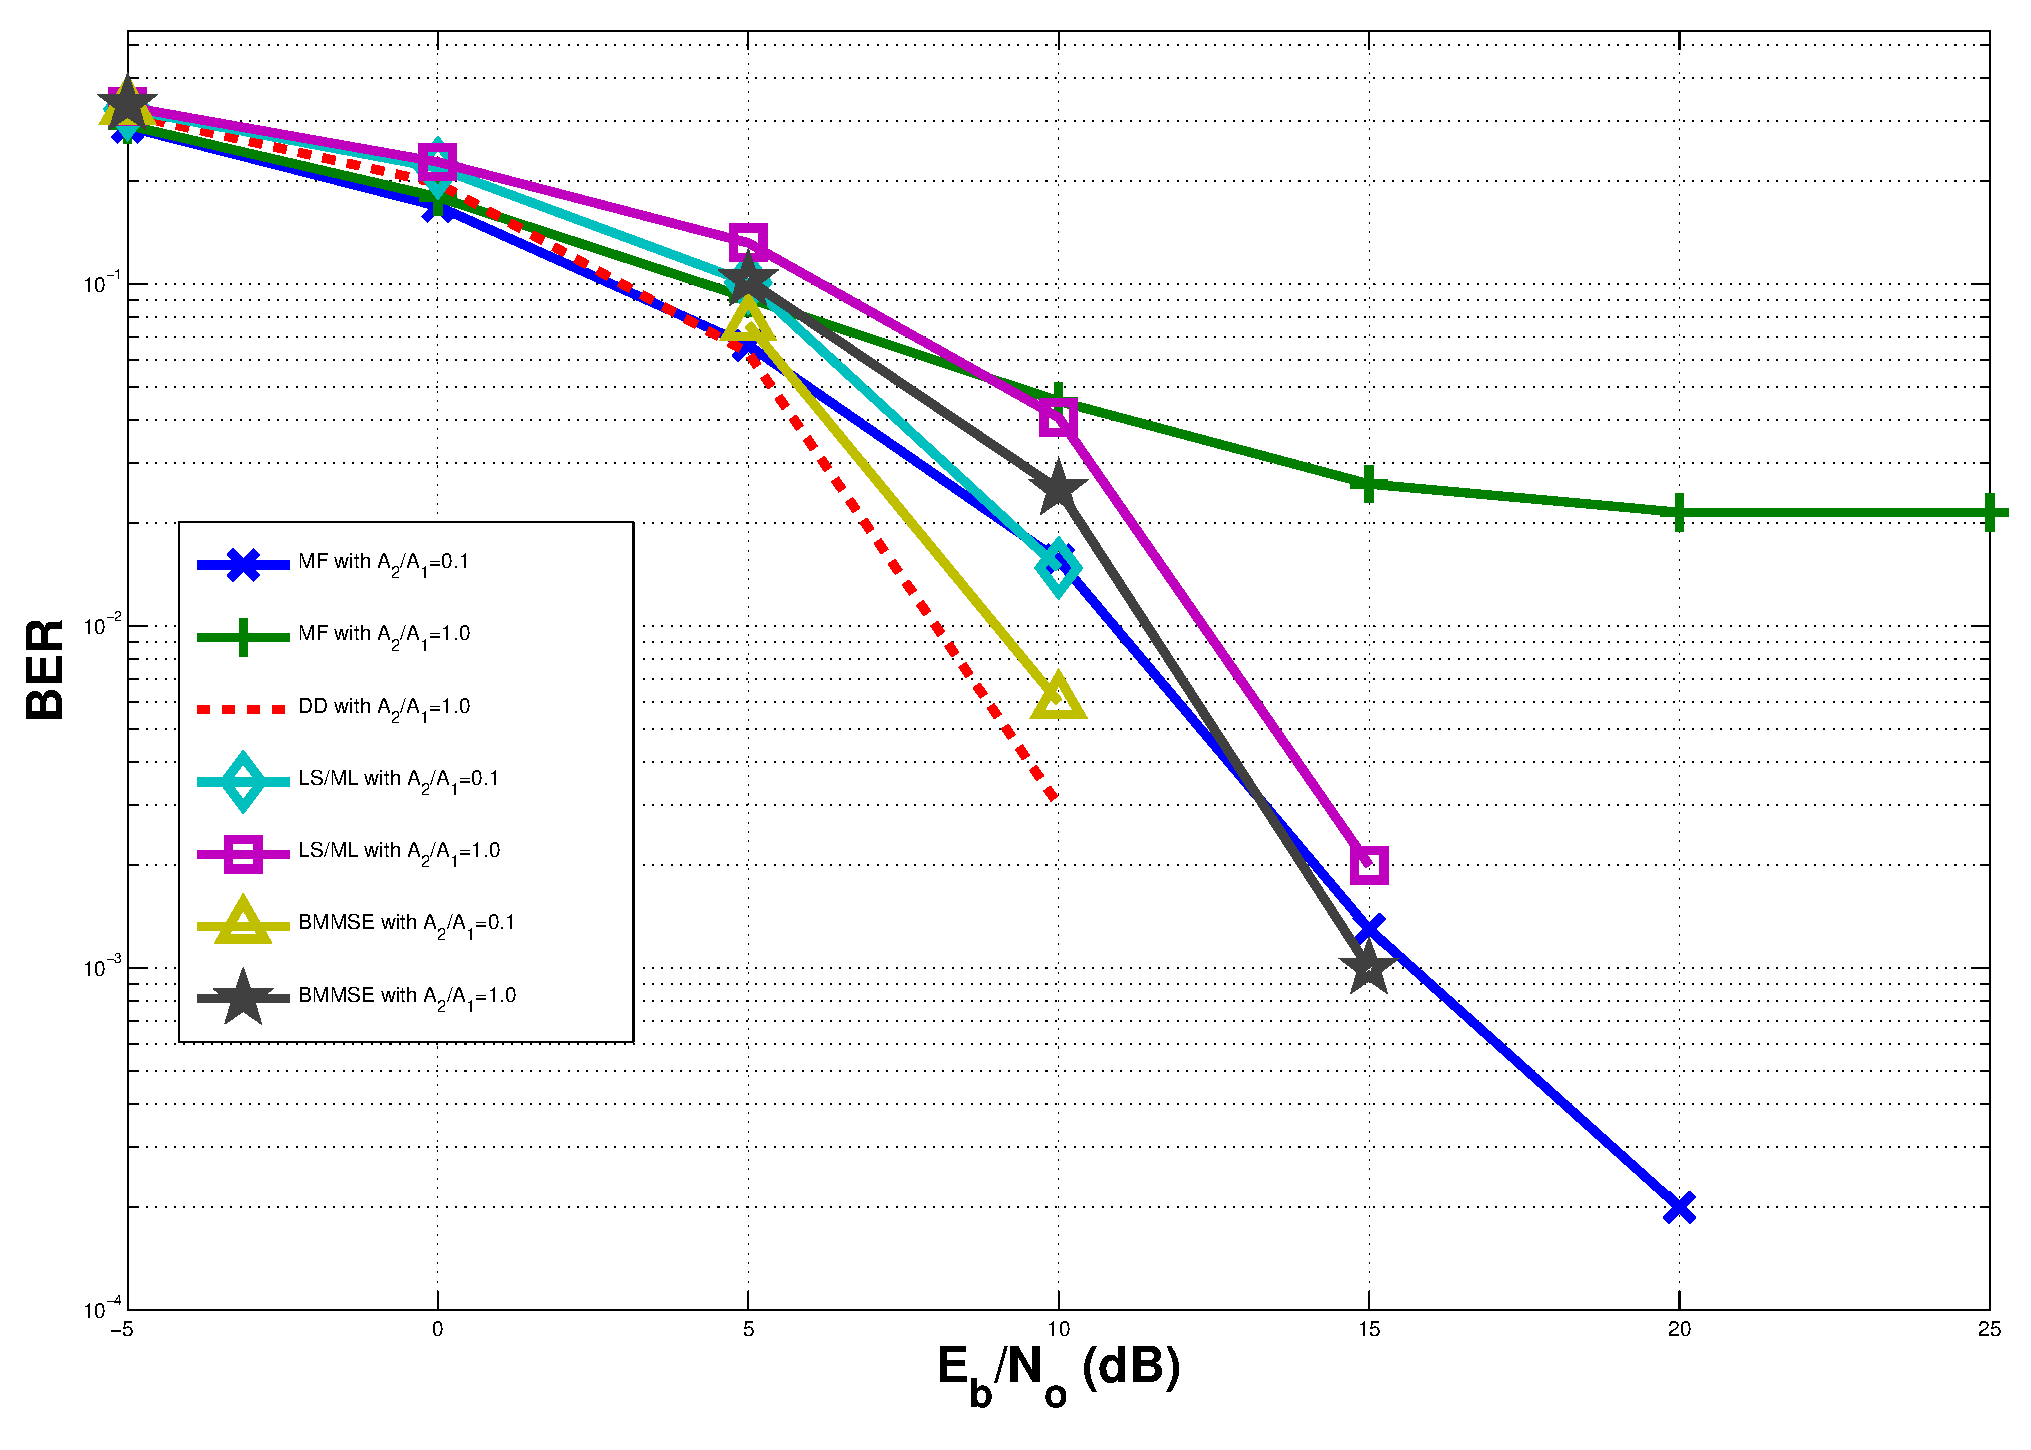
\includegraphics[width=3.2in]{BER_64_32_16_8A1.eps}}
\caption{ The BER of various schemes with low interference against
SNR with $L=64$, $M=32$ and $K=16$.} \label{BER1}
\end{figure}

\begin{figure}
\centerline{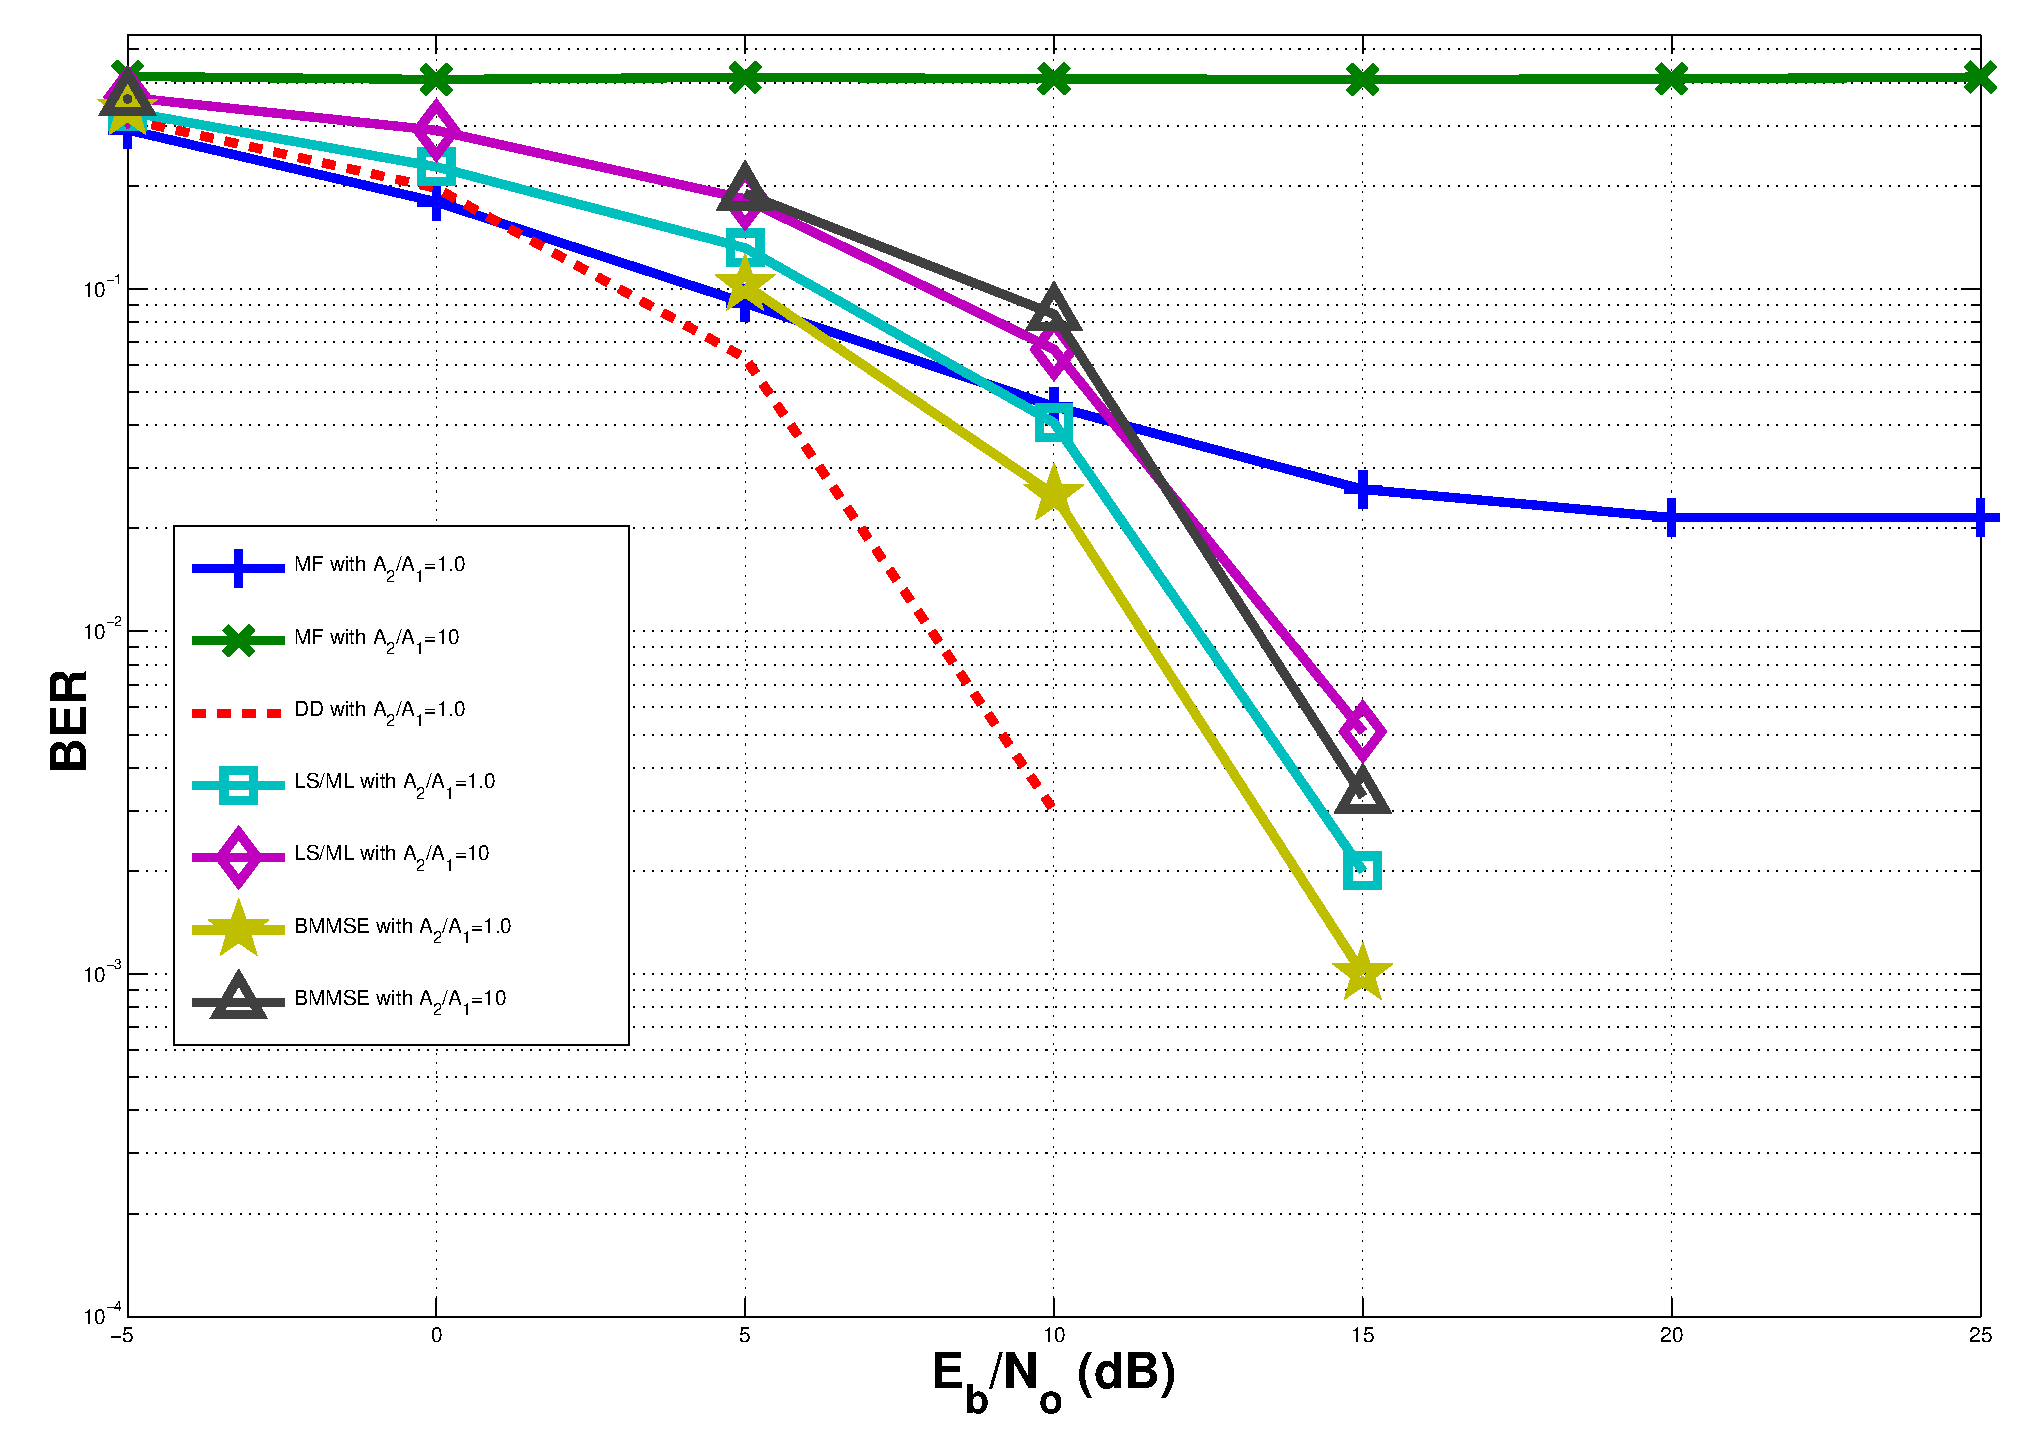
\includegraphics[width=3.2in]{BER_64_32_16_8B1.eps}}
\caption{ The BER of various schemes with high interference
against SNR with $L=64$, $M=32$ and $K=16$.} \label{BER2}
\end{figure}

A single-cell DS/CDMA synchronous multiuser system is simulated. The spreading sequences are random sequences with $L=64$. In
the simulations, previous amplitude estimates are used for the
next detection.  In Fig.~\ref{BER1}, there are $16$ users and $M=32$. From the figure, where the interference is low, the
performance of the blind MMSE detector has the best performance
since it takes advantage of noise estimation. The LS detector
and ML detector are the same and thus have the same performance. From Fig.~\ref{BER2}, the blind
MMSE, LS and ML detectors have similar performance when the
interference is strong. In Fig.~\ref{NFR}, there are two active users
simulated with $M=4$.  The crosscorrelation between these
two users is $\rho=0.25$. We see that the performance of
proposed schemes changes slightly as the near-far
ratio changes.  However, due to the noise enhancement we analyzed before and the fact that the conventional decorrelating detector has knowledge of all users' signature waveforms,
the performance of the proposed detectors is not as good as the conventional decorrelating
detector, which has the best near-far resistance.

\begin{figure}
\centerline{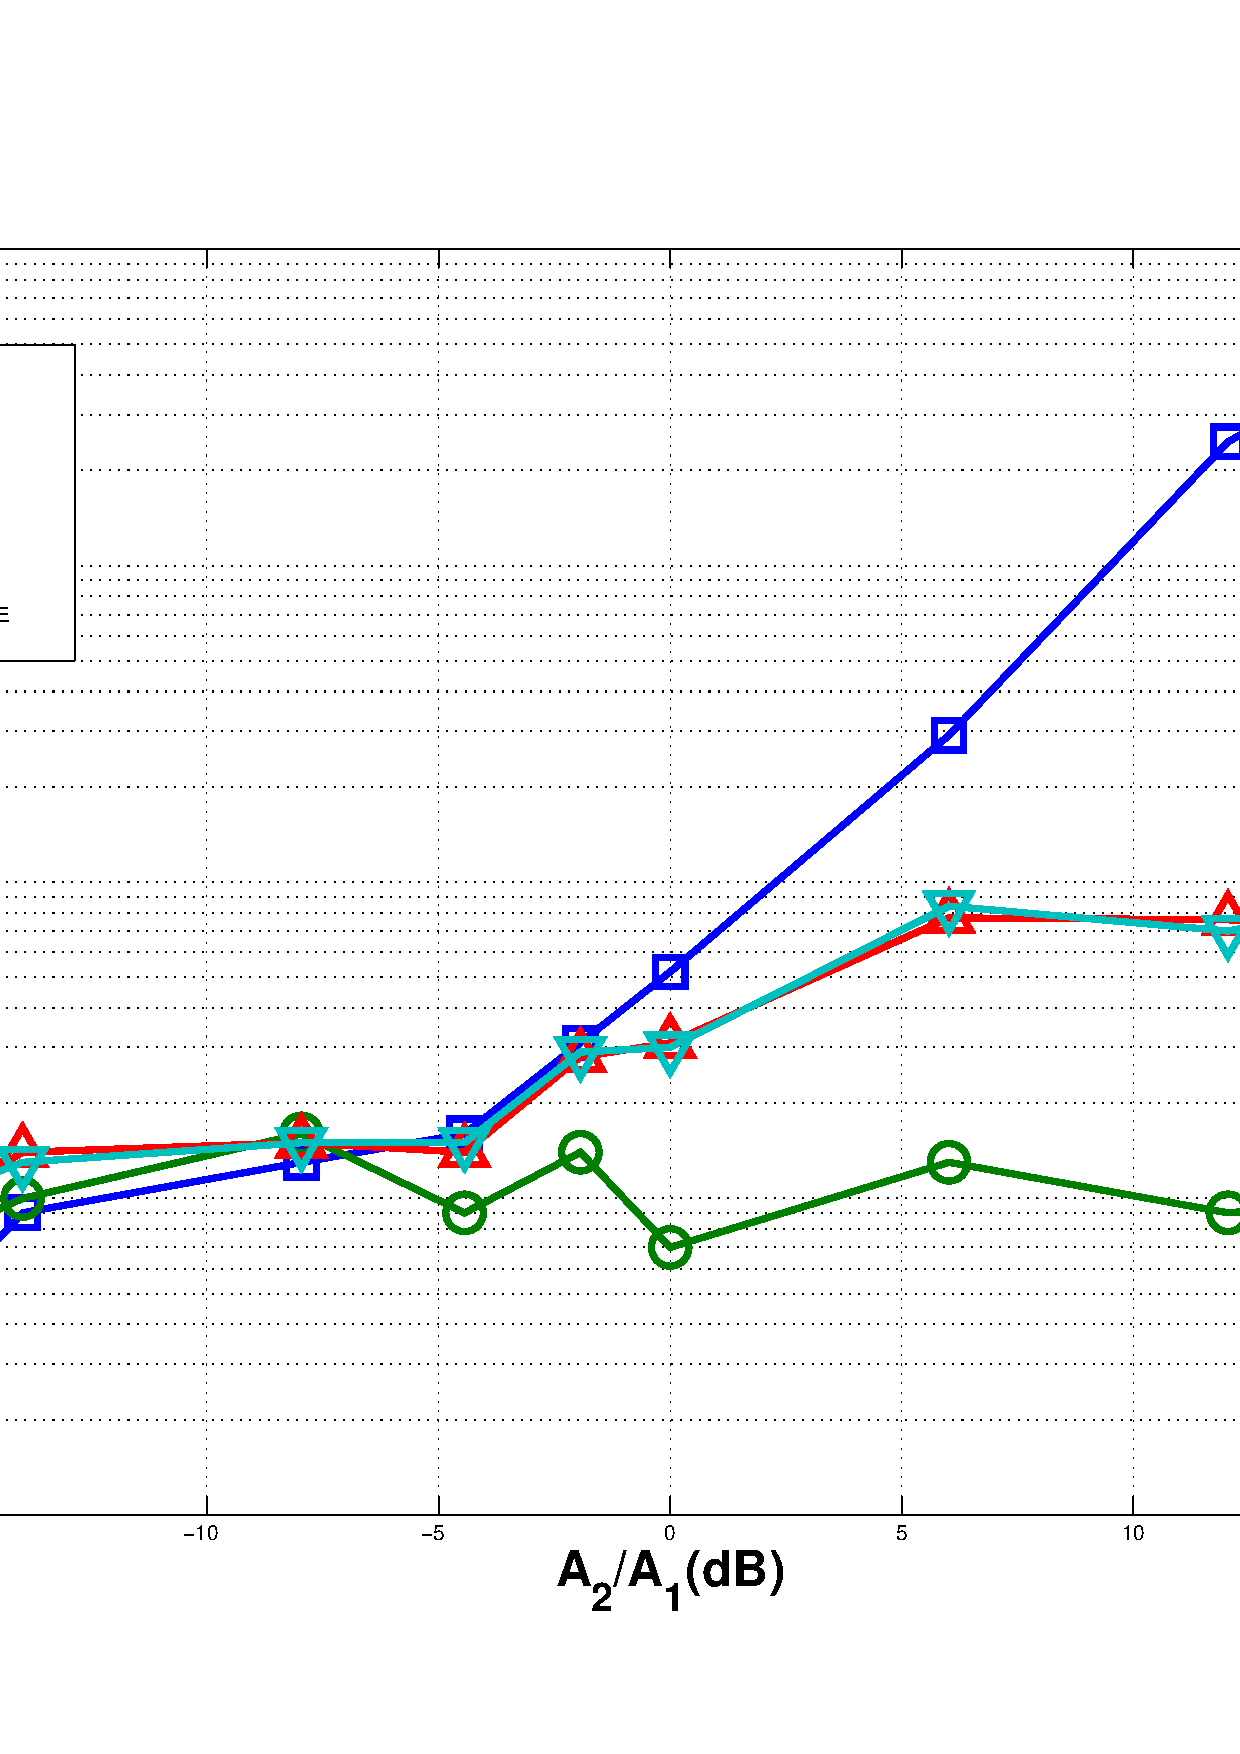
\includegraphics[width=3.2in]{NFR_64_4_2_1B.pdf}}
\caption{ The near-far resistance of various schemes. ${\rm
SNR}=10{\rm dB}$, $\rho=0.25$, $M=4$, $L=64$ and $K=2$.}
\label{NFR}
\end{figure}

\section{Conclusions}

In this paper, we presented a novel approach for blind multiuser
receiver design and compare it with the existing
conventional  receiver and subspace-based receiver designs in
terms of geometric properties, asymptotic multiuser efficiency,
near-far resistance, noise enhancement and the Cram\'{e}r-Rao lower
bound.  The proposed model, which includes previous received signal vectors in the new signature matrix, requires no knowledge of other users' received signal information (either estimated or {\em a priori}) and compares reasonably well in terms of performance with the conventional decorrelating detector.

%\small
\bibliographystyle{ieeetr}
\bibliography{FastBDD,InterferenceCancellation}
\end{document}
